\documentclass[a4paper,12pt]{article}
\usepackage[english,ukrainian,russian]{babel}
\linespread{1}
\usepackage{ucs}
\usepackage[utf8]{inputenc}
\usepackage[T2A]{fontenc}
\usepackage[paper=portrait,pagesize]{typearea}
\usepackage{amsmath}
\usepackage{bigints}
\usepackage{amsfonts}
\usepackage{graphicx}
\usepackage{amssymb}
\usepackage{cancel}
\usepackage{gensymb}
\usepackage{multirow}
\usepackage{rotate} 
\usepackage{pdflscape}
\usepackage{bigstrut}
\usepackage[pageanchor]{hyperref}
\usepackage{chngpage}
\usepackage{fancybox,fancyhdr}
\newcommand\tab[1][1cm]{\hspace*{#1}}
\newcommand{\RomanNumeralCaps}[1]{\MakeUppercase{\romannumeral #1}}
\usepackage[left=20mm, top=20mm, right=15mm, bottom=15mm, nofoot]{geometry}


\begin{document}
    \pagestyle{fancy}
    \fancyhead{}
    \fancyhead[R]{ФІ-12 Завалій Олександр}
    \begin{center}
        \large{\textbf{Міністерство освіти і науки України\\
                Національний технічний університет України\\
                «Київський політехнічний інститут імені Ігоря Сікорського»\\
                Навчально-науковий Фізико-технічний інститут}}\\
        \hfill \break \hfill \break \hfill\break \hfill \break \hfill \break \hfill \break \hfill \break
        \hfill \break \hfill \break \hfill \break
        \begin{center}
            \normalsize{\textbf{ОПЕРАЦІЙНІ СИСТЕМИ\\
            Комп’ютерний практикум\\
            Робота №5}}
        \end{center}
    \end{center}
    \hfill \break \hfill \break \hfill \break \hfill \break \hfill \break \hfill \break \hfill \break
    \hfill \break \hfill \break \hfill \break \hfill \break 
    \begin{flushright}
        \large{ \hspace{35pt} Виконав:\\
            студент групи ФI-12\\
            Завалій Олександр\\} 
        \large{ \hspace{35pt} Перевірив:\\
        Кірієнко О.В.} 
    \end{flushright}
    \hfill \break \hfill \break \hfill \break \hfill \break \hfill \break \hfill \break \hfill \break
    \hfill \break
    \begin{center} \textbf{Київ-2023} \end{center}
    \thispagestyle{empty}

\newpage
    \begin{center}
        \section*{\bfseries{Робота №5.\\
        Процеси в ОС UNIX і керування ними}}
    \end{center}
    \textbf{Мета:} \\
    \hangindent=1.5cm 
    \hangafter=+1 \noindent
    Оволодіння практичними навичками роботи з
    процесами — створення і знищення, керування процесами та їх аналіз \\
    \begin{center}
        \Large{Варіант №5}
    \end{center}
    Зміст індивідуального завдання:
    \begin{enumerate}
        \item Перегляньте список процесів користувача (вас).
        \item Перегляньте повний список процесів, запущених у системі. При цьому гарантуйте збереження інформації від
        "утікання" з екрана (якщо процесів багато). Зверніть увагу на ієрархію процесів. Простежте через поля PID і PPID всю
        ієрархію процесів тільки-но запущеної вами команди, починаючи з початкового процесу init. Зверніть увагу на
        формування інших полів виводу.
        \item Запустіть ще одну оболонку shell. Перегляньте повний список процесів, запущених вами, при цьому зверніть
        увагу на ієрархію процесів і на їхній зв'язок з терміналом. Використовуючи команду kill, завершіть роботу в цій оболонці.
        \item Перегляньте список задач у системі і проаналізуйте їхній стан.
        \item Запустіть фоновий процес командою
        \textbf{find / -name '*c*' -print > file 2> /dev/null \& 8}
        \item Визначте його номер. Відправте сигнал призупинення процесу. Перегляньте список задач у системі і
        проаналізуйте їхній стан. Продовжить виконання процесу. Знову перегляньте список задач у системі і проаналізуйте 
        його зміну. Переведіть процес в активний режим, а потім знову у фоновий. Запустіть цей процес із пріоритетом 5.
        \item Виведіть на екран список усіх процесів, запущених не користувачем root.
        \item Організуйте виведення на екран календаря \textbf{2015} року через 1 хвилину після поточного моменту часу.
        \item Організуйте періодичне (щоденне) видалення в домашньому каталозі усіх файлів з розширенням *.bak і *.tmp.
    \end{enumerate}

\newpage
    \begin{center}
        \Large{Task \RomanNumeralCaps{1}}
    \end{center}
    \textbf{Перегляньте список процесів користувача (вас).}
    \begin{figure}[h!]
        \begin{minipage}[h]{1\linewidth}
            \centering
            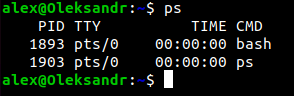
\includegraphics[width=0.6\linewidth]{Prt sc/Figure_1.png}  
        \end{minipage}
    \end{figure}
    \begin{center}
        \Large{Task \RomanNumeralCaps{2}}
    \end{center}
    \textbf{Перегляньте повний список процесів, запущених у системі. При цьому гарантуйте збереження інформації від
    "утікання" з екрана (якщо процесів багато). Зверніть увагу на ієрархію процесів. Простежте через поля PID і PPID всю
    ієрархію процесів тільки-но запущеної вами команди, починаючи з початкового процесу init. Зверніть увагу на
    формування інших полів виводу.}
    \begin{figure}[h!]
        \begin{minipage}[h]{1\linewidth}
            \centering
            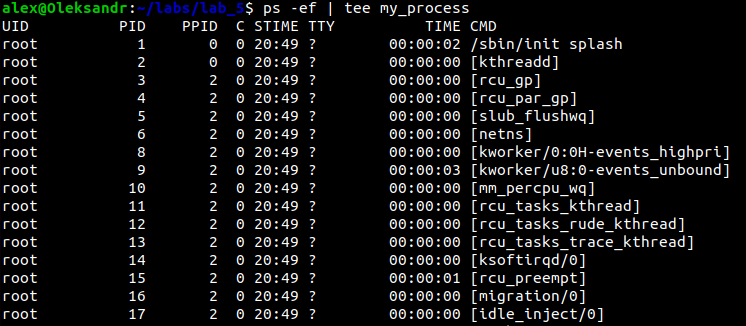
\includegraphics[width=0.8\linewidth]{Prt sc/Figure_2_1.png}  
        \end{minipage}
    \end{figure}
    \begin{figure}[h!]
        \begin{minipage}[h]{1\linewidth}
            \centering
            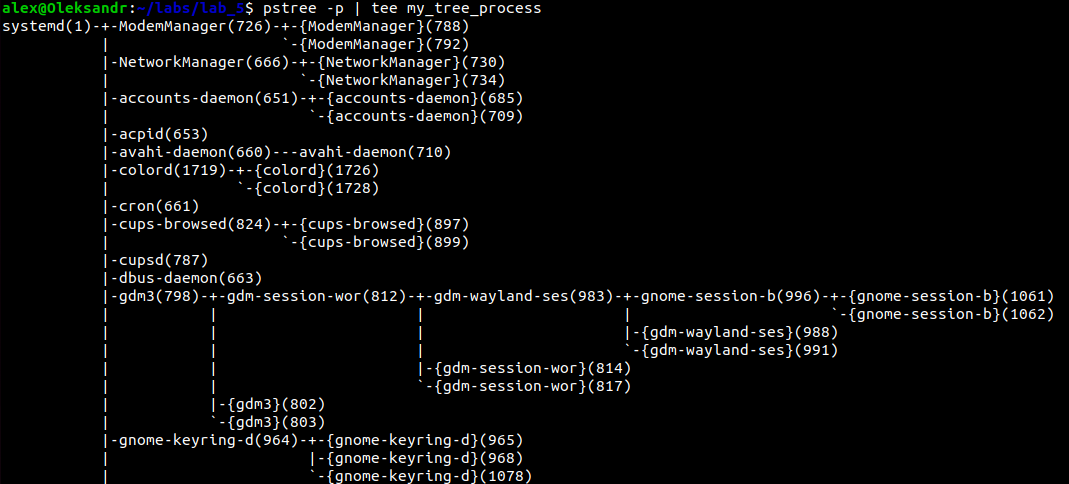
\includegraphics[width=0.8\linewidth]{Prt sc/Figure_2_2.png}  
        \end{minipage}
    \end{figure}

\newpage
    \begin{center}
        \Large{Task \RomanNumeralCaps{3}}
    \end{center}
    \textbf{Запустіть ще одну оболонку shell. Перегляньте повний список процесів, запущених вами, при цьому зверніть
    увагу на ієрархію процесів і на їхній зв'язок з терміналом. Використовуючи команду kill, завершіть роботу в цій оболонці.}
    \begin{figure}[h!]
        \begin{minipage}[h]{1\linewidth}
            \centering
            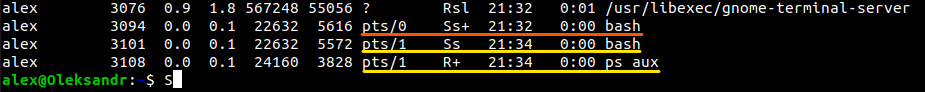
\includegraphics[width=0.8\linewidth]{Prt sc/Figure_3_1.png}  
        \end{minipage}
    \end{figure}
    \begin{figure}[h!]
        \begin{minipage}[h]{1\linewidth}
            \centering
            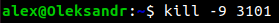
\includegraphics[width=0.6\linewidth]{Prt sc/Figure_3_2.png}  
        \end{minipage}
    \end{figure}
    \begin{center}
        \Large{Task \RomanNumeralCaps{4}}
    \end{center}
    \textbf{Перегляньте список задач у системі і проаналізуйте їхній стан.}
    \begin{figure}[h!]
        \begin{minipage}[h]{1\linewidth}
            \centering
            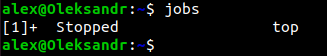
\includegraphics[width=0.6\linewidth]{Prt sc/Figure_4.png}  
        \end{minipage}
    \end{figure} \\
    Процес призупинено.
    \begin{center}
        \Large{Task \RomanNumeralCaps{5}}
    \end{center}
    Запустіть фоновий процес командою
    \textbf{find / -name '*c*' -print > file 2> /dev/null \& 8}
    \begin{figure}[h!]
        \begin{minipage}[h]{1\linewidth}
            \centering
            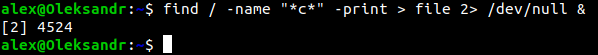
\includegraphics[width=0.6\linewidth]{Prt sc/Figure_5.png}  
        \end{minipage}
    \end{figure}
    \begin{center}
        \Large{Task \RomanNumeralCaps{6}}
    \end{center}
    \textbf{Визначте його номер. Відправте сигнал призупинення процесу. Перегляньте список задач у системі і
    проаналізуйте їхній стан. Продовжить виконання процесу. Знову перегляньте список задач у системі і проаналізуйте 
    його зміну. Переведіть процес в активний режим, а потім знову у фоновий. Запустіть цей процес із пріоритетом 5.}
    \begin{figure}[h!]
        \begin{minipage}[h]{1\linewidth}
            \centering
            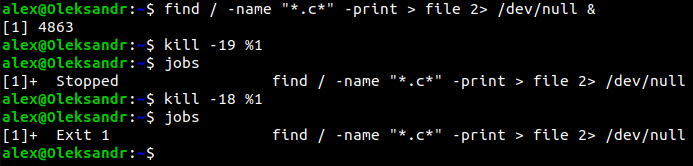
\includegraphics[width=0.6\linewidth]{Prt sc/Figure_6_1.png}  
        \end{minipage}
    \end{figure} \\
    Конмадою kill -19 \%1 можна призупинити процес. Тому бачимо, що 1 процес має атрибут Stopped.
    Після цього виконання процесу продовжено конмадою kill -18 \%1.
    Далі бачимо, що процес завершує свою роботу.

\newpage
    \begin{figure}[h!]
        \begin{minipage}[h]{1\linewidth}
            \centering
            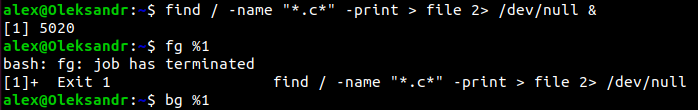
\includegraphics[width=0.6\linewidth]{Prt sc/Figure_6_2.png}  
        \end{minipage}
    \end{figure}
    \begin{figure}[h!]
        \begin{minipage}[h]{1\linewidth}
            \centering
            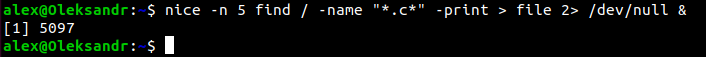
\includegraphics[width=0.6\linewidth]{Prt sc/Figure_6_3.png}  
        \end{minipage}
    \end{figure}
    \begin{center}
        \Large{Task \RomanNumeralCaps{7}}
    \end{center}
    \textbf{Виведіть на екран список усіх процесів, запущених не користувачем root.}
    \begin{figure}[h!]
        \begin{minipage}[h]{1\linewidth}
            \centering
            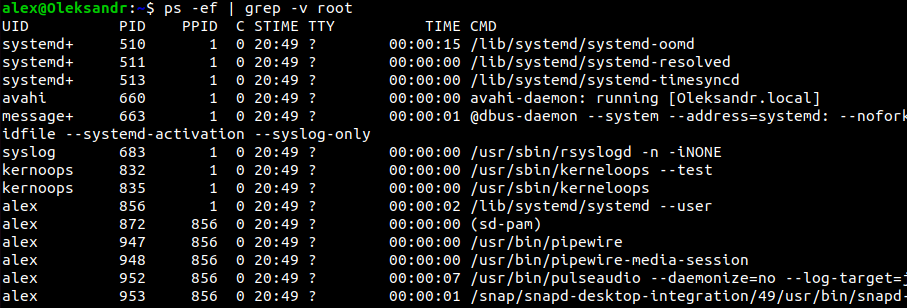
\includegraphics[width=0.6\linewidth]{Prt sc/Figure_7.png}  
        \end{minipage}
    \end{figure}
    \begin{center}
        \Large{Task \RomanNumeralCaps{8}}
    \end{center}
    \textbf{Організуйте виведення на екран календаря \textbf{2015} року через 1 хвилину після поточного моменту часу.}
    \begin{figure}[h!]
        \begin{minipage}[h]{1\linewidth}
            \centering
            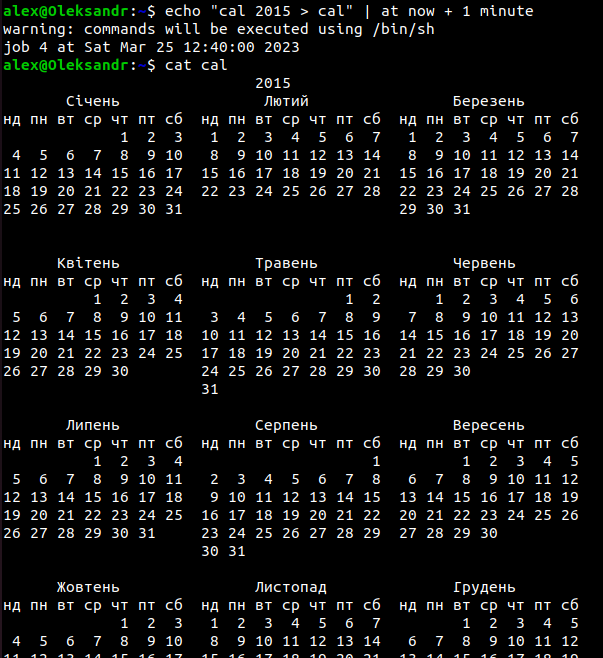
\includegraphics[width=0.6\linewidth]{Prt sc/Figure_8.png}  
        \end{minipage}
    \end{figure}

\newpage
    \begin{center}
        \Large{Task \RomanNumeralCaps{9}}
    \end{center}
    \textbf{Організуйте періодичне (щоденне) видалення в домашньому каталозі усіх файлів з розширенням *.bak і *.tmp.}
    \begin{figure}[h!]
        \begin{minipage}[h]{1\linewidth}
            \centering
            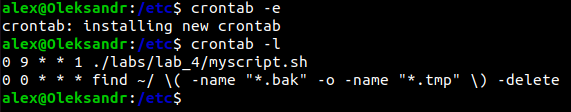
\includegraphics[width=0.6\linewidth]{Prt sc/Figure_9.png}  
        \end{minipage}
    \end{figure}
    \begin{center}
        \Large{Висновки}
    \end{center}

    Процеси у Linux є основною одиницею виконання програмного забезпечення. Кожен процес має свій унікальний ідентифікатор PID, який дозволяє ідентифікувати процеси.
    Також за цим ідентифікатором можна звертатись до процесу.

    Щоб отримати інформацію про:
    \begin{itemize}
        \item Процеси, що виконуються в системі.
        \item Подивитись використані ресурси системи.
        \item Залежності між процесами.
    \end{itemize}
    Використовують команди ps, top та htop. 

    Команди kill, pkill та killall дозволяють зупиняти процеси використовуючи PID або імена процесів.

    Також є можливість запускати процеси у фоновому режимі, використовуючи символ \&. Це потрібно для того, щоб звільнити термінал.
    Щоб при закритті терміналу процес продовжував своє виконання використовують nohup.

    Тобто контроль процесів є ключовою функцією операційної системи, оскільки він забезпечує можливість моніторингу та керування цих самих процесів.
    Сюда можна також віднести управління ресурсами системи, ефективності роботи, забезпечення безпеки, діагностика та виконання програм.

\end{document}